% ------------------------------------------------------------------------------
% TYPO3 Version 9.1 - What's New - Chapter "Wijzigingen voor  integrators" (Dutch Version)
%
% @author	Michael Schams <schams.net>
% @license	Creative Commons BY-NC-SA 3.0
% @link		http://typo3.org/download/release-notes/whats-new/
% @language	English
% ------------------------------------------------------------------------------
% LTXE-CHAPTER-UID:		3a9852ea-e2360d9d-1ff5eec1-a7de3f9f
% LTXE-CHAPTER-NAME:	Wijzigingen voor  integrators
% ------------------------------------------------------------------------------

\section{Wijzigingen voor integrators}
\begin{frame}[fragile]
	\frametitle{Wijzigingen voor integrators}

	\begin{center}\huge{Hoofdstuk 2:}\end{center}
	\begin{center}\huge{\color{typo3darkgrey}\textbf{Wijzigingen voor integrators}}\end{center}

\end{frame}

% ------------------------------------------------------------------------------
% LTXE-SLIDE-START
% LTXE-SLIDE-UID:		ce032961-e6659e3b-1706a1dd-1ba54372
% LTXE-SLIDE-ORIGIN:	31b70474-edcc2a8a-d4a5fd3d-58734dc5 English
% LTXE-SLIDE-TITLE:		EXT:impexp - Maximum Number Of Records Restriction Removed
% LTXE-SLIDE-REFERENCE:	Deprecation-83592-ImpexpRemovedMaximumNumberOfRecordsRestriction
% ------------------------------------------------------------------------------

\begin{frame}[fragile]
	\frametitle{Wijzigingen voor  integrators}
	\framesubtitle{Importeren/Exporteren}

	Diverse aanpassingen zijn doorgevoerd in de systeem extensie \texttt{impexp}:

	\begin{itemize}
		\item Restrictie "maximaal aantal records" is verwijderd\newline
			\smaller
				De optie om slechts een maximum aantal records te exporteren is verwijderd
				bij het exporteren van pagina's of records.
			\normalsize

		\item Restrictie "maximale bestandsgrootte" is verwijderd\newline
			\smaller
				Wanneer bestanden worden geëxporteerd met de "Export" functie, is het nu niet meer mogelijk
				om alleen bestanden te exporteren van een bepaalde maximale grootte.
			\normalsize

		\item Afhandelingsgrootte verwijderd\newline
			\smaller
				Bij het exporteren of importeren van pagina's, records en bestanden werd de groote naar het exportbestand
				geschreven en bij de import gecontroleerd.
				Deze wijziging heeft geen impact voor redacteuren.
			\normalsize

	\end{itemize}

\end{frame}

% ------------------------------------------------------------------------------
% LTXE-SLIDE-START
% LTXE-SLIDE-UID:		4b2e0f86-fc334073-c574153e-f575580d
% LTXE-SLIDE-ORIGIN:	0504ca33-7c23eff4-93a728fa-bd911c92 English
% LTXE-SLIDE-TITLE:		Redirect Functionality Moved To Redirects Module
% LTXE-SLIDE-REFERENCE:	83638-RedirectFunctionalityMovedFromSys_domainToRedirectsModule
% ------------------------------------------------------------------------------

\begin{frame}[fragile]
	\frametitle{Wijzigingen voor  integrators}
	\framesubtitle{Redirect functionaliteit}

	\begin{itemize}
		\item Optie om een redirect in te stellen wanneer een domein werd toegevoegd aan een specifieke pagina of
		    paginaboom, is verwijderd.
		\item Het instellen van redirects kan nu worden gedaan in de nieuwe module\newline
			\textbf{Site Beheer} \textrightarrow \textbf{Redirects}
	\end{itemize}

	\begin{figure}
		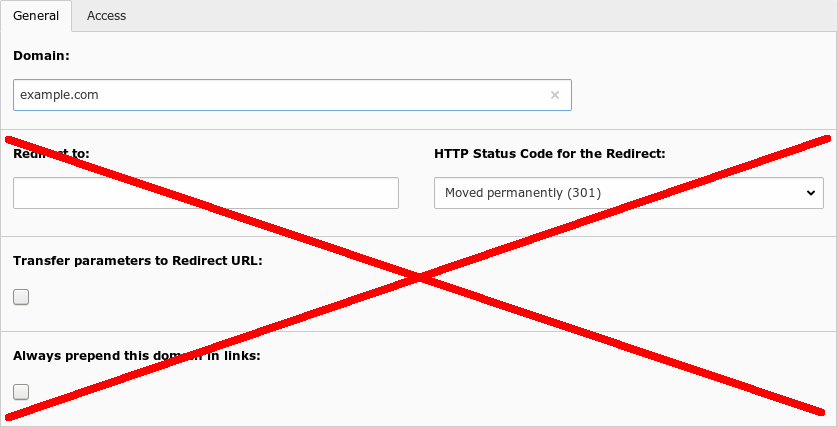
\includegraphics[width=0.6\linewidth]{ChangesForIntegrators/RedirectFunctionalityMovedToRedirectsModule.png}
	\end{figure}

\end{frame}

% ------------------------------------------------------------------------------
